
\begin{document}

\chapter{Introduction}

\label{chapter:introduction}

People detection and tracking is the process of identifying and following people in an environment. Knowing where people are is important for human traffic~\cite{yang_count_people} and behaviour analysis~\cite{seer_pedestrian_behaviour, arar_gaze_estimation}. There is also a growing interest in human-robot interactions~\cite{mutlu_human_robot_interaction}. It is likely that in the future there will be many social robots interacting with people and with other robots, thus requiring them to navigate around a stochastic environment. These robots must be able to avoid obstacles and track people persistently, either through a centralized control (orchestration) or decentralized, autonomous cooperation (choreography). There is ongoing research in using mobile robots for tracking people~\cite{choi_indoor_robots, munaro_tracking_within_groups_with_mobile_robot, munaro_tracking_2, glas_people_tracking_robot_localization, satake_stereo_robot}. The current work focuses on tracking people under occlusion.

\section{Problem Statement}
\label{sec:introduction_problem_statement}

The efficacy of tracking algorithms often depends on the quality of initial detection results. The current work leverages Kinect sensor's ability to identify people from a depth map. This allows the researcher to focus on the problem of tracking.

Tracking moving objects is non-trivial. There are many sources of tracking errors, including raw sensor data noise, illumination levels, changing backgrounds, and occlusion. Tracking in real-life scenarios are even harder. The environment is unpredictive and complex, often consisting of multiple people. A crowded environment with complex human interactions gives rise the the problem of occlusion.

Occlusion occurs when the tracked target is masked by other objects in the scene. The masked target would not exist in the field of view of one or more cameras. If a person were occluded, his precise joint positions and movements would be unknown. Resolving the problem of occlusion would provide any tracking system with more spatial and physiological information about the tracked people.

There are two types of occlusions: static and dynamic. They are defined as:

\begin{description}
  \item[Static occlusion] Occlusion caused by stationary objects in the environment 
  \item[Dynamic occlusion] Occlusion caused by people interactions in the environment
\end{description}

A simple instance of the problem is illustrated in Figure~\ref{fig:occlusion_problem}. In the figure, both skeletons are invisible to the front Kinect but visible to the side Kinect. They are occluded by the red obstacle. When they step out of the obstacle into the views of both Kinects, the system should merge the skeletons of the same person from different perspectives. The main objective of the project is to avoid occlusion by extending the field of view of the system. The proposed algorithm would combine depth sensor information from multiple Kinects to achieve this goal.

\begin{figure}[!h]
  \centering
  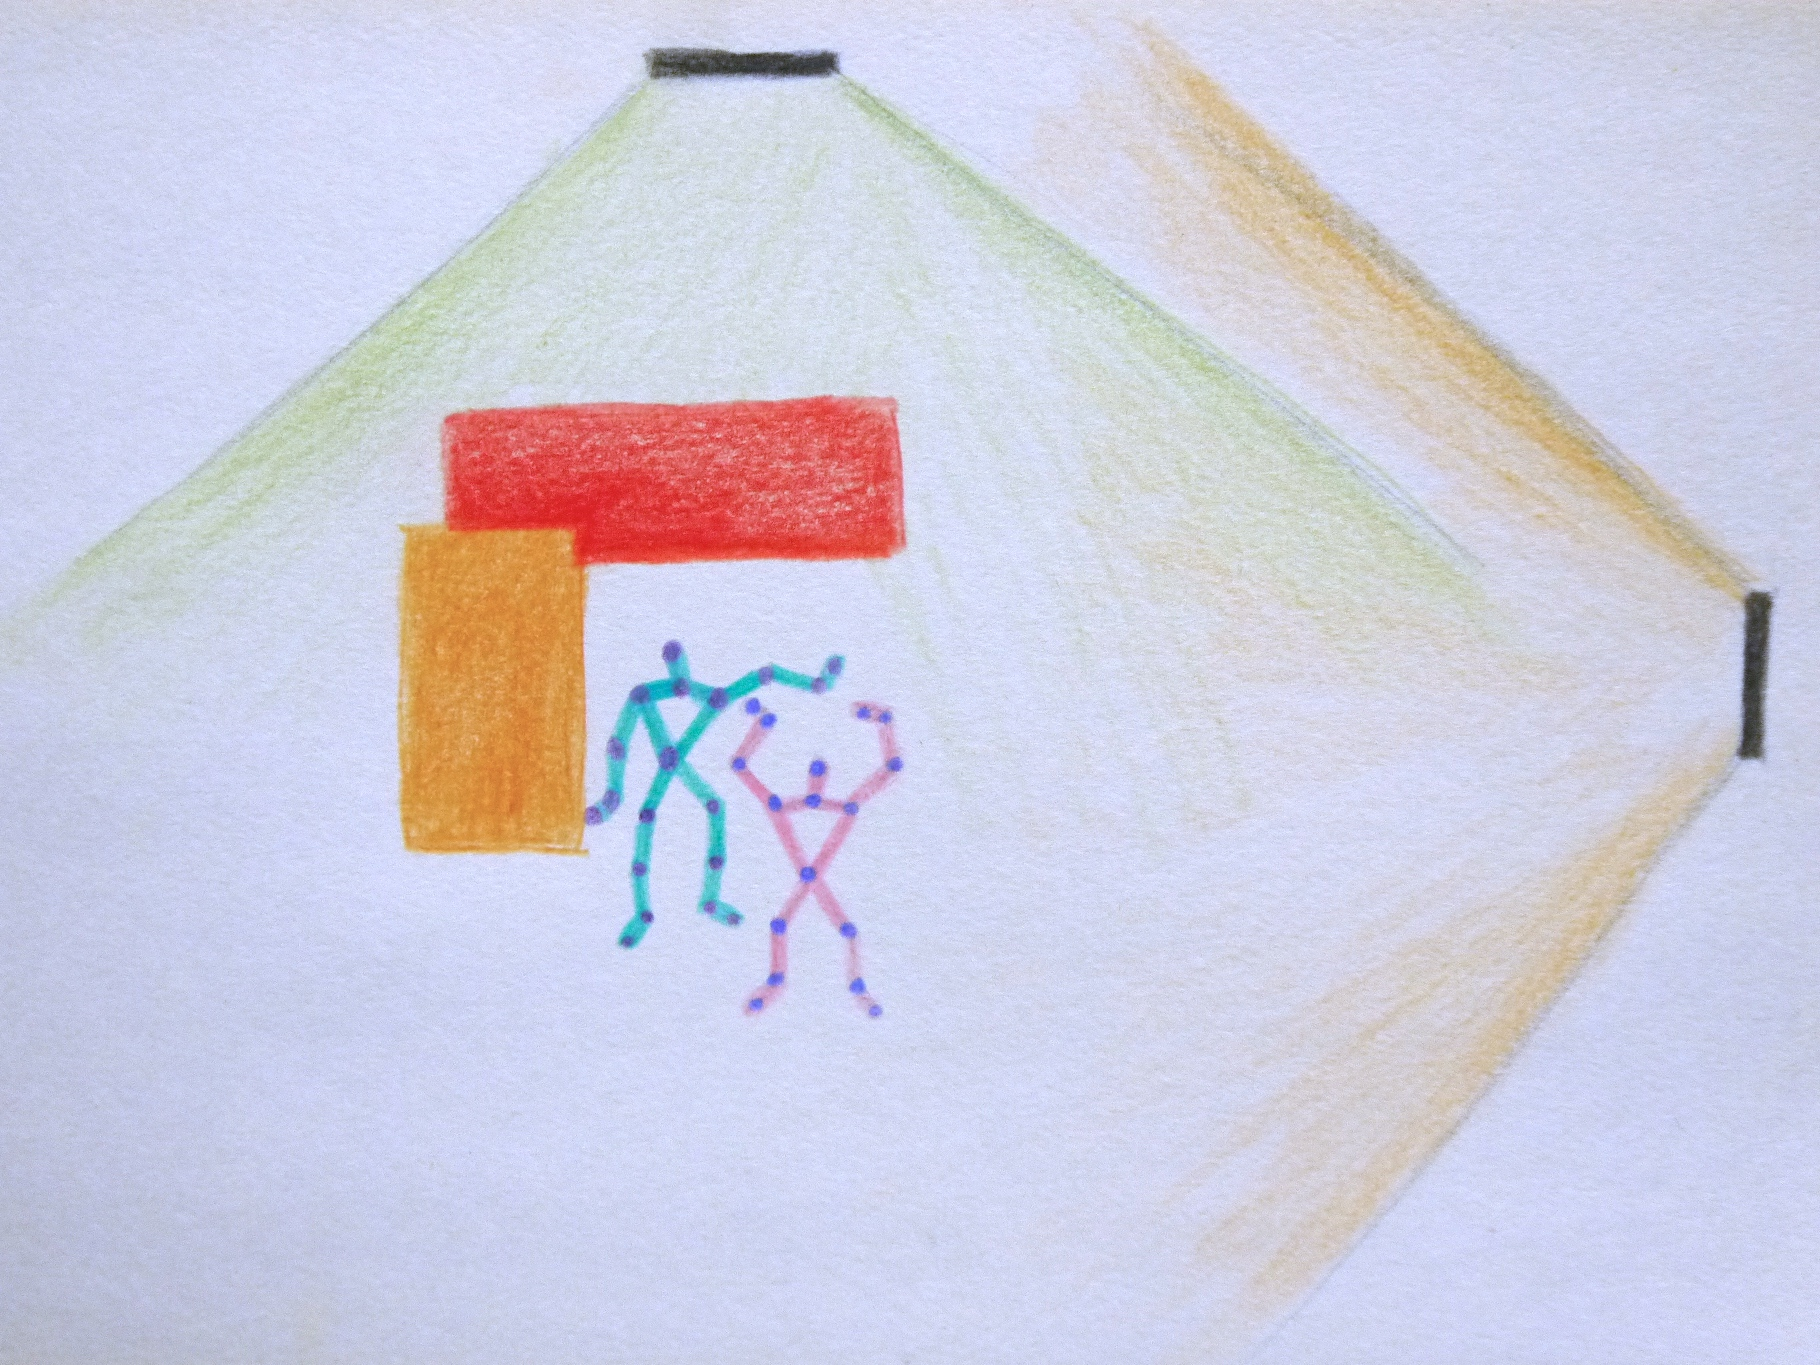
\includegraphics[width=0.8\linewidth]{figs/occlusion_problem}
  \caption{The occlusion problem}
  \label{fig:occlusion_problem}
\end{figure}

The current work addresses the occlusion problem by extending the field of view with multiple Kinects. The field of view, also known as FOV, is the extent to which the scene is observable through the camera. By extending the field of view, the system will have a more complete view of the environment in 3D space that was not available with a single camera.

\section{Contributions}
\label{sec:introduction_contributions}

The contributions of the current work are\ldots

\begin{enumerate}
  \item Replicate, validate, and extend current research
  \item A Kinect BodyFrame serialization library
  \item A Kinect client-server framework
  \item Track people with multiple Kinects
  \item Integrate joints information from multiple Kinects to resolve the occlusion problem
  \item User studies showing the strengths and weaknesses of the current system
\end{enumerate}

\section{Kinect}
\label{sec:introduction_kinect}

Kinect is a commodity depth sensor for body motion capturing and tracking. It provides depth and RGB streams at 30 frames per second~\cite{kinect_sensor_specs}, allowing for the possibility of robust tracking using these devices.

The current work uses the Kinect BodyFrame stream, which includes the skeletal information of the people in the sensor's field of view. The complete API reference for the Kinect v2 SDK is accessible at \url{https://msdn.microsoft.com/en-us/library/windowspreview.kinect.aspx}.

The system manipulates coordinates in the Kinect Camera Space. These coordinates are 3D points, consisted of the x, y, and z components, in meters. The origin of the coordinate system at (0, 0, 0) is ``located at the center of the IR sensor on Kinect"~\cite{microsoft_kinect_coordinates}. The x axis grows to the left of the sensor, the y axis grows upward from the sensor, and the z axis grows outward from the direction the sensor (See Figure~\ref{fig:kinect_camera_space}).

\begin{figure}[!h]
  \centering

  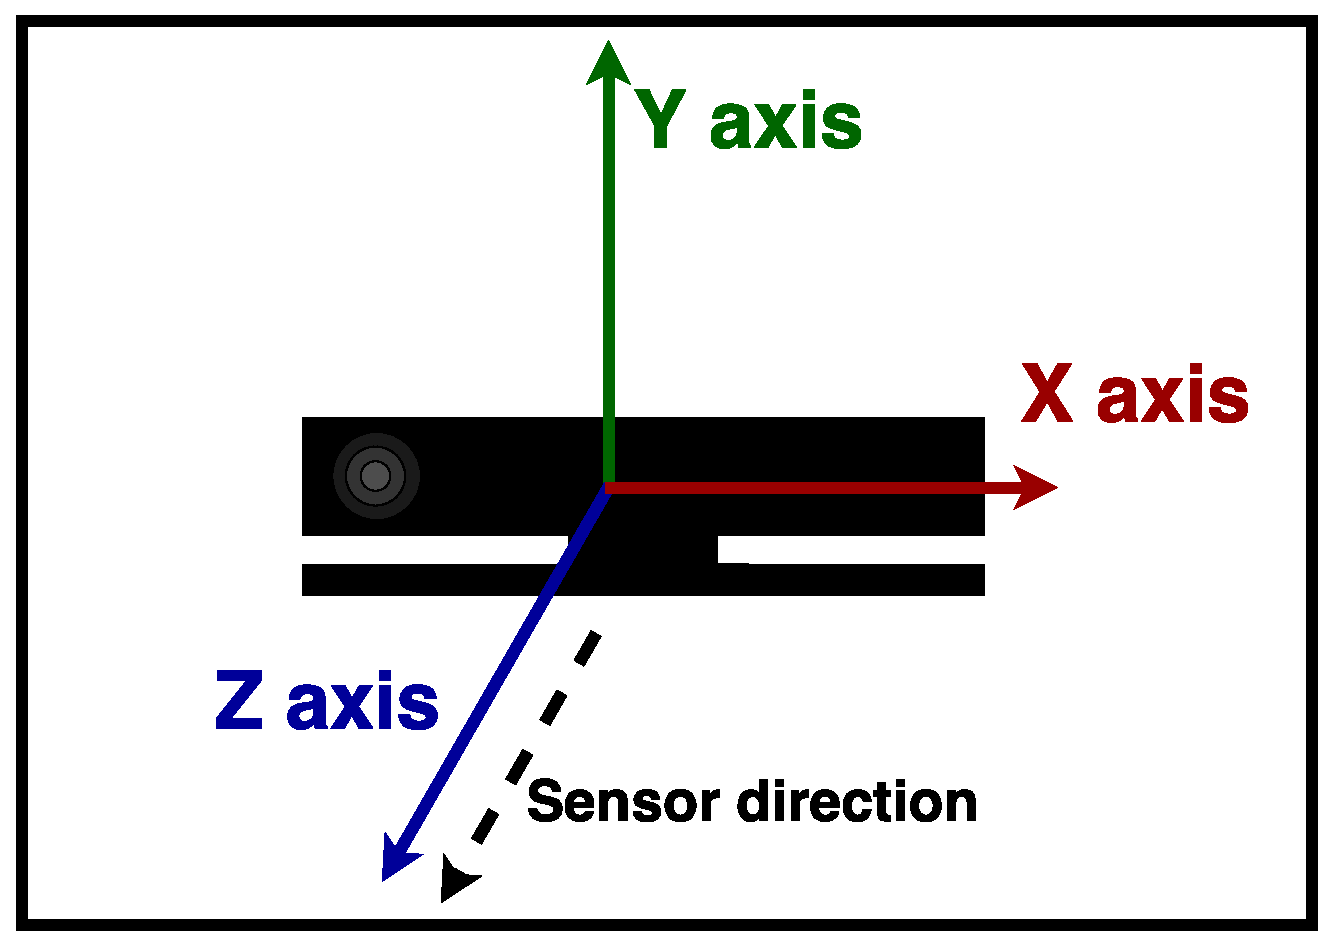
\includegraphics[width=0.5\linewidth]{figs/kinect_camera_space}
  
  \caption{The Kinect Camera Space}
  
  \label{fig:kinect_camera_space}
\end{figure}

\end{document}
